\documentclass[conference]{IEEEtran}
\IEEEoverridecommandlockouts
% The preceding line is only needed to identify funding in the first footnote. If that is unneeded, please comment it out.
\usepackage{cite}
\usepackage{amsmath,amssymb,amsfonts}
\usepackage{algorithmic}
\usepackage{graphicx}
\graphicspath{ {./images/} }
\usepackage{textcomp}
\usepackage{xcolor}
\def\BibTeX{{\rm B\kern-.05em{\sc i\kern-.025em b}\kern-.08em
    T\kern-.1667em\lower.7ex\hbox{E}\kern-.125emX}}
\begin{document}

\title{DENTIFY THE PLANT AND DISEASE BASED ON THE LEAF PROVIDED\\
{\footnotesize Data Mining and Machine Learning II}
}

\author{\IEEEauthorblockN{Pedro Acosta}
\IEEEauthorblockA{\textit{School of Computing} \\
\textit{National College of Ireland}\\
Dublin, Ireland \\
x21138745@student.ncirl.ie}
\and
\IEEEauthorblockN{Brendan O’Dwyer}
\IEEEauthorblockA{\textit{School of Computing} \\
\textit{National College of Ireland}\\
Dublin, Ireland \\
x21145172@student.ncirl.ie}
\and
\IEEEauthorblockN{Femi Adeboye}
\IEEEauthorblockA{\textit{School of Computing} \\
\textit{National College of Ireland}\\
Dublin, Ireland \\
x21137684@student.ncirl.ie}
\and
\IEEEauthorblockN{Antonio Milian y Albacar}
\IEEEauthorblockA{\textit{School of Computing} \\
\textit{National College of Ireland}\\
Dublin, Ireland \\
x19172125@student.ncirl.ie}
}

\maketitle

\begin{abstract}
Plant disease identification, techniques results.
\end{abstract}

\begin{IEEEkeywords}
Convolutional Neural Networks 
\end{IEEEkeywords}

\section{Introduction}
%The remainder of the 1stpage and up to 1 column of2nd page  

%Provide a motivation for your work. Present and discuss the researchquestion(s) / objective(s) of the paper and (optionally) provide a concise overview of the following sections (max 1-2 lines for each) 

%Motivation 

Emerging technologies and diverse applications make it possible nowadays to prevent or early detect challenging situations where consequences impact not only financially but in the quality of life of people. Nowadays geopolitical conflicts urge all stakeholders in society to reduce errors and waste of resources, especially on food, the current project aims to contribute and make possible the early detection through images of the type of plant and serves to early detect diseases on them. From small farmers that use their mobile phones to industrialized companies taking images with drones, the main objective is to make available the results and techniques from this study for them to be integrated or embedded as part of a simple, complex or wider solution that includes not only indoor analysis but also outdoor data. 

 %Discussion Research questions and objectives 

Since one of the core objectives of the project is to provide a reliable model that identifies plants and diseases based on outdoor images, this adds a level of complexity due to the nature of the situation, noise or information factors such as illumination, background, disease signs distributed randomly along with different type of plants around, all contribute to a right application of XXXXXXXXXXXXX 

%Overview following sections 

XXXXXXXXXXX 

Identifying plant diseases at an early stage allows home gardeners, and rural and industrial farmers to take action and reduce crop loss. In the same way, the usage of basic technology such as smart phones as well as more sophisticated and emerging technologies such as drones are leading to consideration of alternatives that could allow stakeholders to identify plant diseases using the technologies already mentioned. This project will allow for the identification of the type of plant between apple, tomato and pepper detecting if they are healthy or carrying some type of disease. This model could be used as part of a system where images can be the input either by uploading them via PC, or using mobile phones, it could also receive images from drones or pictures taken in laboratories. The results could be used as a part of a more complex system that applies pesticides wherever a crop disease is identified. 

In this study we train convolutional neural network models using images of leaves of diseased plants to identify the plant disease. The research question we are attempting to answer in this study is: how do CNN models trained on images of leaves of diseased plants in order to classify plant disease compare when trained using laboratory data, outdoor data and both combined and tested on laboratory and outdoor data? There are two hypotheses in this study:
\begin{itemize}
\item[•]The performance of a CNN model trained with both laboratory and augmented outdoor data should perform substantially better than a model trained with both laboratory and outdoor data without augmentation when tested on laboratory and outdoor data. 
\item[•]The performance of a CNN model trained with a combination of laboratory and augmented outdoor data should perform substantially better than a model trained with laboratory data alone when tested on outdoor data.
\end{itemize}  

 

This report is structured as follows: the Related Work section provides a review of related literature. The Methodology section describes our methodology. The Results and Evaluation section presents our results and evaluates our method. The Conclusions and Future Work section discusses our conclusions and proposed future work. The References section provides the references in this report.

\section{Related work}
1 page with citations into 20 or more works  

This should not only summarise related work, but also critically evaluate the strengths and weaknesses of the cited works with respect to the topic under study, i.e. how well/badly does the cited work answer your question(s), what aspects are useful to consider, what are the limitations? You should also discuss any foundational papers that either substantiate your study design or upon which you are building. ne part of the entire proceedings, and not as an independent document. Please do not revise any of the current designations. 

\section{Methodology }

The CRoss Industry Standard Process for Data Mining (CRISP-DM) data mining methodology has been followed in this study. The data mining lifecycle is described by the six phases of this methodology. It is a flexible and iterative process. Phases can be revisited as the project progresses.
\begin{figure}[htbp]
\centerline{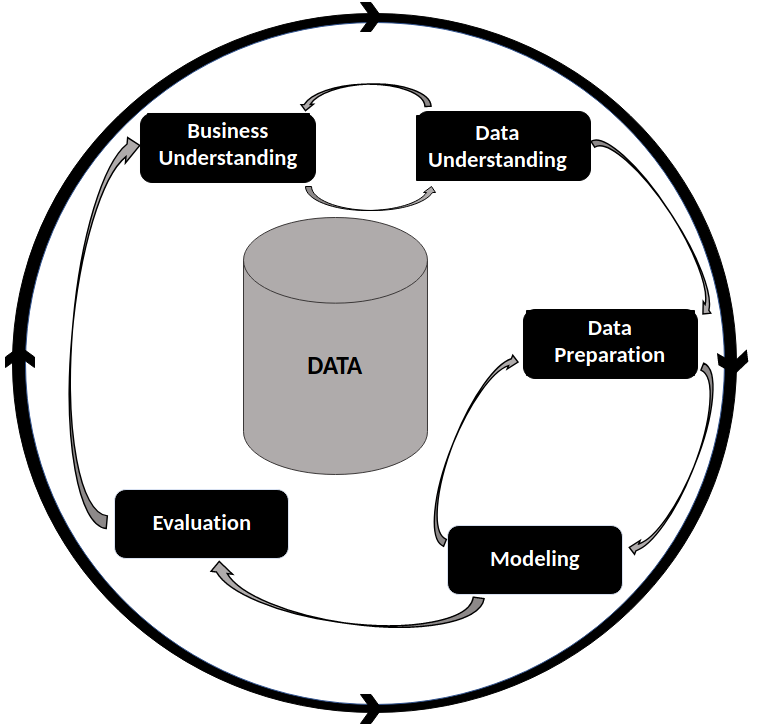
\includegraphics[width=8.5cm]{CRISP_DM_no deployment.png}}
\caption{    The phases of the CRISP-DM cycle. Business understanding, data understanding, data preparation, modelling and evaluation in this case there is not deployment phase as the evaluation is the output.}
\label{fig}
\end{figure}
This study will involve training different models and as a result phases will be revisited repeatedly. Business understanding is the first phase in CRISP-DM. The data mining goals are determined in this phase and an understanding of the objectives and requirements of the project developed. In the introduction the objectives of the study have been outlined. The business understanding phase is addressed through these objectives as well as through the understanding developed from the related work publications. In the remainder of this report a description of the other CRISP-DM phases is provided


\subsection{Data Understanding}\label{AA}
Exploration and collection of data is carried out in the CRISP-DM data understanding phase. An understanding of the data is obtained as well as an understanding of how the objectives can be addressed through the data. 

Two datasets are used in this study. The first, PlantVillage\cite{kaggledatasetPlantville}, contains images of leaves of diseased and healthy plants with the associated labels. The images are taken indoors in laboratory conditions. The data are made available through the PlantVillage online platform. In total there are over 50,000 images of crop plant leaves that are infected or healthy. There are 14 different types of plant species with 38 classes in total. Each class corresponds to a plant-disease pair. 

The second dataset, Plant Doc\cite{kaggledatasetPlantDoc}, is for detecting plant disease from images. Unlike the first dataset the images are taken outdoors rather than in laboratory conditions. There are 2,598 images in total. There are 13 species of plants in total with 17 disease classes. The data were obtained by scraping images from webpages and annotating them. 

The PlantVillage dataset contains coloured, segmented and greyscale versions of each image. The coloured versions of the images were used. In the case of Plant Doc only colour images are provided. For the 13 classes used in this study in total 18,317 images from the PlantVillage dataset were used.  
\subsection{Data Preparation}
This phase of CRISP-DM involves manipulating data acquired in the data understanding phase in order to prepare it for the modelling phase. The datasets were explored using Python. The feature selection is based on the commonalities between the previously described datasets. Three plant species present in both the PlantVillage and Plant Doc datasets were selected apple, pepper and tomato. In total there are 13 disease classes for these plants common to both datasets. Below the classes and the number of items per class and dataset. 

These classes are apple scab leaf, apple healthy leaf, apple rust leaf, bell pepper leaf healthy, bell pepper leaf spot, tomato early blight leaf, tomato septoria leaf spot, tomato leaf healthy, tomato leaf bacterial spot, tomato leaf late blight, tomato leaf mosaic virus, tomato leaf yellow virus and tomato mold leaf, more details for the classes in Table I.
\begin{table}[htbp]
\caption{Data Sets used}
\begin{center}
\begin{tabular}{|c|c|c|c|c|}
\hline
\textbf{Classes}&\multicolumn{4}{|c|}{\textbf{Data sets}} \\
\cline{2-5} 
\textbf{Ojbective} & \textbf{\textit{Indoor}}& \textbf{\textit{Outdoor}}& \textbf{\textit{O.Augmented}} & \textbf{\textit{Combined}} \\
\hline
apple scab &630&87&1307&1937 \\
\hline
apple healthy &275&89&1392&1667\\
\hline
apple rust &1645&91&1325&2970\\
\hline
bell pepper healthy &997&71&1355&2352\\
\hline
bell pepper spot &1478&61&1581&3059\\
\hline
tomato early blight &2127&107&1256&3383\\
\hline
tomato septoria  &1591&62&1392&2983\\
\hline
tomato healthy &1000&83&1379&2379\\
\hline
tomato bacterial &1771&148&1272&3043\\
\hline
tomato late blight &1909&111&1306&3215\\
\hline
tomato mosaic  &373&54&1131&1504\\
\hline
tomato yellow virus &5357&75&1172&6529\\
\hline
tomato mold &952&91&1444&2396\\
\hline
\multicolumn{5}{l}{$^{\mathrm{a}}$Original Data set classes and values.}
\end{tabular}
\label{tab1}
\end{center}
\end{table}

Two test datasets were created. The first uses only images from the dataset of indoor laboratory data. The second consists of images taken outdoors from the Plant Doc dataset. For each of the PlantVillage and Plant Doc datasets the remaining data are assigned randomly to training datasets, validation datasets and datasets used for tuning hyperparameters. 72\% of the data are assigned to the training datasets, 20\% are assigned to the validation datasets and 8\% are assigned to the datasets for tuning hyperparameters. \

All images were adjusted to have the dimensions 240 pixels by 240 pixels for InceptionResNetv.2 and to 224 x224 when using MobileNetv.2. The PlantVillage dataset has more images for each class than the Plant Doc dataset. As a result of this data augmentation techniques were applied to the Plant Doc dataset. These techniques included rotation, shearing, zooming, flipping horizontally and adjusting the brightness range.The data were preprocessed. The pixel values are rescaled. . 
\subsection{Modelling}
    The model typology to be used to analyse the data is CNN, to take advantage of the properties of the models in imagge recongintionModelling techniques are used to build and assess models in the CRISP-DM modelling phase. A batch size of 32 was used. As convolutional layers two types are taken into consideration, Inception ResNet, in this case the pretrained convolutional neural network Inception-ResNet-v2 was used for transfer learning. Weights trained on the ImageNet dataset, which has one thousand classes and 1.4 million images, were used. On top of this model a new classifier is added. The layers of the base convolutional model are frozen. The second type is MobileNet. In addition to Inception-ResNet-v2 the pretrained convolutional neural network MobileNet V2 was also used for transfer learning. The data were again preprocessed in preparation for use with the MobileNet V2 model. Weights trained on the ImageNet dataset were used. As before a new classifier was added on top of this model and the layers of the base convolutional model were frozen.  
\subsection{Hyperparameter Optimisation}
Adding to the convolutional layers described the optimizers Adam and Adagrad were also tested. Combining the different values of convolutional layers and optimizers several models are proposed as potential candidates.\

 The models are passed to a build model function in which several parameters are proposed for the rate of drop on the and the learning rate. A few values are provided for both variables. The optimization is centered in finding the best values for drop rate and from the learning rate. The model with the Convolution layer is frozen and a range of values proposed for both variables. The values for learning rates ranging from 0.01 to 0.00001, and the drop rates used range from 0.1 to 0.2.\

From the algorithm point of view, he library keras tuner has been used to ascertain the optimal values. From keras tuner, the Hyperband tuning algorithm is chosen. The algorithm has the championship bracket approach, running the models and choosing only the half best performers to be carried onto the next epoch.  This approach is faster and guarantees better results than a simple Grid optimization approach.  The keras tuner implementation has been run for 6 epochs in each trial, obtaining the optimal learning rate for each model as well as the optimal number of epochs.  Accuracy over the validation is the metric used to find the best parameter values. The goal is to decide which model’s architecture render the best validation accuracy and continue with that model through the fine-tuning process.\ 

Same methodology has been used for the three different implementations; the values gathered have subsequently used in the tested models. The three models were trained using the three different data sets, Indoors, Outdoor and Combined. The outdoor model is using the Outdoor data set, with the augmentation images for training. \

 

Applying the Hyperparameter optimization over the datasets the below results are obtained, 

\subsection{Model using the Indoor images}
Applying the Hyperparameter tuning to the indoor data set, the model that offers the best results has a convolutional layer based on MobileNet v.2 with the Adam optimizer, which gives not only better accuracy at 96.9\% but is also 4 times faster than the ResNet v.2 (94.5\%) with the same optimizer. Trying Adagrad as optimizer for MobileNet v.2  the accuracy obtained 95\%, so the model chosen for the indoor data set is MobileNet v.2 with Adam optimizer with the parameters obtained from the hyperparameter tuner. 

The images are transformed into 224 x 224 pixels, to match with MobileNet requirements. The drop rate is of 0.2 and the learning rate 0.0001 as provided by the Keras tuner algorithm. The dense layer has 1280 nodes and 16,653 trainable parameters,the ones after the Dense layer as show in figure 2.
\begin{figure}[htbp]
\centerline{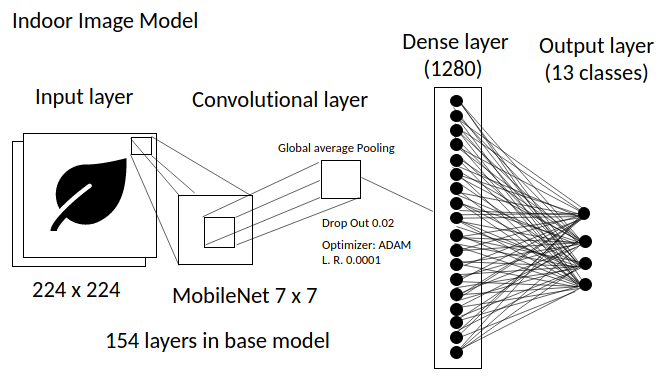
\includegraphics[width=8.5cm]{ModelIndoorsMobileNet.png}}
\caption{MobileNet Indoor model schema.}
\label{fig}
\end{figure}
    The model is the trained for ten epochs before fine tuning. The accuracy obtained was 90.75\% for the training subset and 93\% for the validation subset as show in figure x. The model was trained for another five epochs for fine tuning. For fine tuning as series of modifications were introduced, the learning rate was reduced by a factor of 10 and the layers from 100 upwards were used in fine-tuning the model. 
    
\begin{figure}[htbp]
\centerline{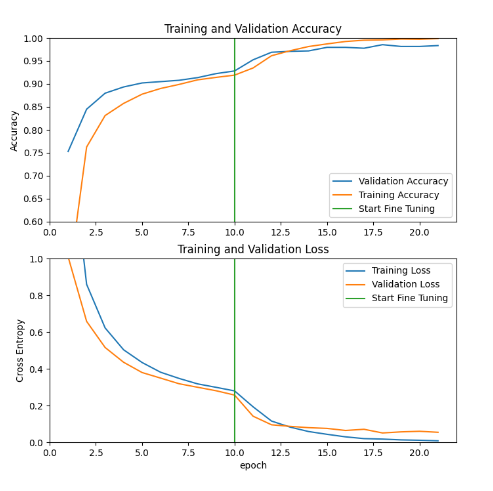
\includegraphics[width=8.5cm]{ModelIndoorsMobileNetEpochsAccuracychart.png}}
\caption{Model MobileNet v.2 with Adam Optimizer Indoor dataset for Accuracy and Cross Entropy.}
\label{fig}
\end{figure}

%\begin{figure}[htbp]
%\centerline{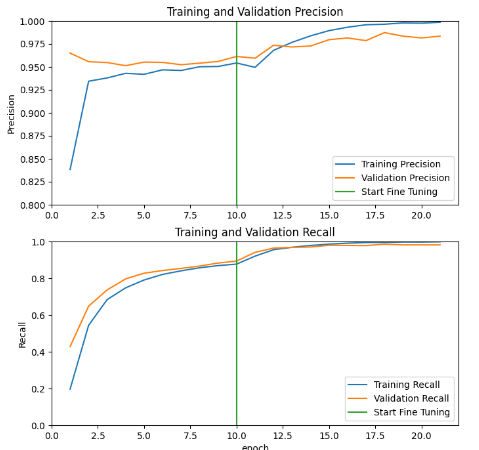
\includegraphics[width=8.5cm]{ModelIndoorsMobileNetPrecRecchart.png}}
%\caption{Model MobileNet v.2 with Adam Optimizer Indoor dataset for Precision and Recall.}
%\label{fig}
%\end{figure}

For this model the total number of parameters was again 2,274,637, but in this case 1,878,093 of these were trainable. e fine tuning epochs a big increase on the accuracy is observed, where on the epoch 12 the accuracy of the validation and the one from the training subset are similar at 97.4\%. For reference, in\cite{saleem2020plant} for classification of crop disease the authors carry out a comparison of deep learning architectures and optimisers. The best classification accuracy for the validation set was 99.81\% obtained using the Adam optimiser to train the Xception architecture. \
Similar behaviour can be observed using the metrics Precision and Recall, when around the 11 or 12 epoch the validation and training subsets provide similar values. 

\subsection{Model using the Outdoor images}
%A convolutional neural network model was trained on the PlantVillage indoor laboratory images and tested on both the test dataset of indoor images and the test dataset of outdoor images. Another CNN model was trained on the Plant Doc outdoor images and tested on both the indoor and outdoor test datasets. The indoor laboratory images and outdoor images were merged into a combined training dataset and a model was trained on this dataset and tested on both the indoor and outdoor test datasets. An additional model was trained on the augmented Plant Doc outdoor images dataset and tested on both test datasets. The augmented outdoor images dataset was merged with the indoor laboratory images dataset and a model trained on the combined dataset and tested on both test datasets. (to edit)

Applying the Hyperparameter tuning to the outdoor data set, the model that offers the best results uses the pretrained convolutional neural network MobileNet v.2 with the Adam optimiser, which gives not only better accuracy at 89.7\% but is also 4 times faster than the ResNet v.2 (82.8\%) with the same optimiser. Trying Adagrad as the optimiser for MobileNet v.2 the accuracy obtained is 83.3\%, so the model chosen for the outdoor data set is MobileNet v.2 with Adam optimiser with the parameters obtained from the hyperparameter tuner. 

The images are transformed into 224 x 224 pixels, to match with MobileNet requirements. The drop rate is of 0.1 and the learning rate is 10-5 as provided by the Keras tuner algorithm. The dense layer has 1280 nodes and 16,653 trainable parameters. 

The model is then trained for ten epochs before fine tuning. The accuracy obtained was 40.9\% for the training subset and 45.2\% for the validation subset as shown in Figure x. The model was trained for another ten epochs for fine tuning. For fine tuning a series of modifications were introduced. The learning rate was reduced by a factor of 10. As the model we are training is much larger we reduce the learning rate. Our model may overfit quickly if at this stage we don’t adjust the learning rate. The layers from 100 upwards were used in fine-tuning the model. For this model the total number of parameters was again 2,274,637, but in this case 1,878,093 of these were trainable. In the fine-tuning epochs, a big increase on the accuracy is observed, where on the epoch 13 the accuracy of the validation and the one from the training subset are similar. The best validation accuracy obtained was 97.9\%.
\begin{figure}[htbp]
\centerline{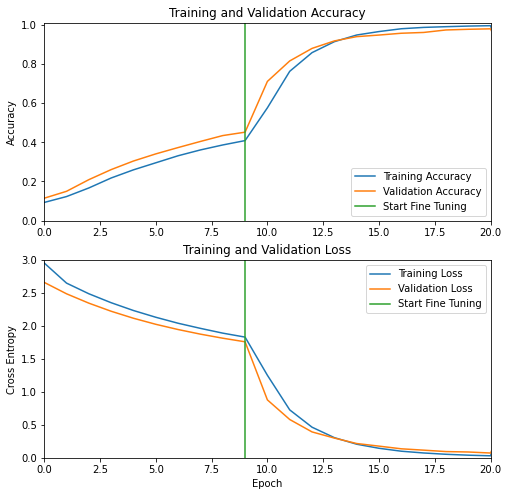
\includegraphics[width=8.5cm]{ModelOutdoorsMobileNetEpochsAccuracychart.png}}
\caption{For model trained on the augmented Plant Doc outdoor data with transfer learning using the pretrained MobileNet V2 CNN with fine tuning and Adam optimiser training and validation accuracy are plotted against epoch number in the upper panel. In the lower panel the training and validation loss are plotted against epoch number.}
\label{fig}
\end{figure}

%\begin{figure}[htbp]
%\centerline{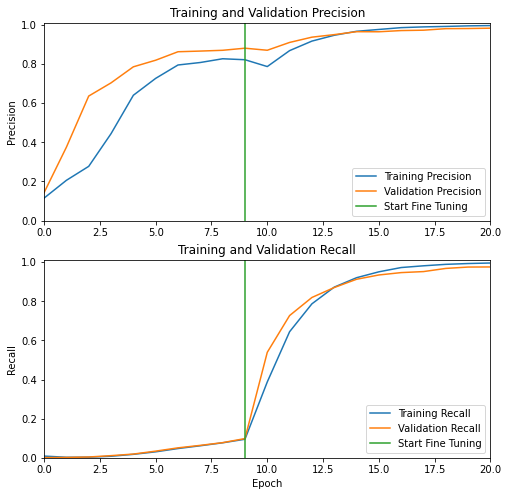
\includegraphics[width=8.5cm]{ModelOutdoorsMobileNetOtherMetricschart.png}}
%\caption{For model trained on the augmented Plant Doc outdoor data with transfer learning using the pretrained MobileNet V2 CNN with fine tuning and Adam optimiser training and validation precision are plotted against epoch number in the upper panel. In the lower panel the training and validation recall are plotted against epoch number}
%\label{fig}
%\end{figure}

Similar behaviour can be observed using the metrics precision and recall, when around epoch 13 the validation and training subsets provide similar values.
 
\begin{figure}[htbp]
\centerline{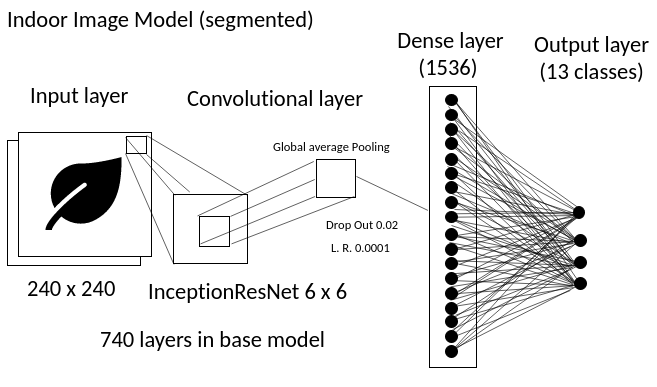
\includegraphics[width=8.5cm]{ModelIndoorsResNet.png}}
\caption{InceptionResNetv.2 Indoor Segmented model schema.}
\label{fig}
\end{figure}

\subsection{Combined data model}

The same methodology is applied to a dataset that combines the pictures from the outdoor and indoor data sets. The outdoor data includes the augmented added items in the training subset. From the data set thus conformed a train data set of 33394 images is extracted and further divided into 30052 for the training side and 3339 for the validation. Using these images to compare the different model proposed, InceptionResNetV2 with Adam as optimizer, renders the best accuracy at 6 epochs for the optimized values of 0.1 drop and 0.00001 learning rate of 85.56\%. MobileNet with Adagrad  for the same number of epochs and optimized parameters, Learning Rate, 0.01 and drop, 0.1 renders better accuracy at 87.24\%. The best accuracy is obtained using the MobileNet with Adam, with the optimised values of 0.0001 for the learning rate and 0.2 for the drop at 90.35\%. It is also worth to acknowledge that the MobileNet instances were 4 times faster than the InceptionResNetV2, which would make them more compelling even with similar results. \

Using the best model from the hyperparameter tunning phase, it is trained for 10 epochs in a first phase where the layers are frozen for training, therefore only the parameters after the dense layer are trainable, 16,653 in total.\
\begin{figure}[htbp]
\centerline{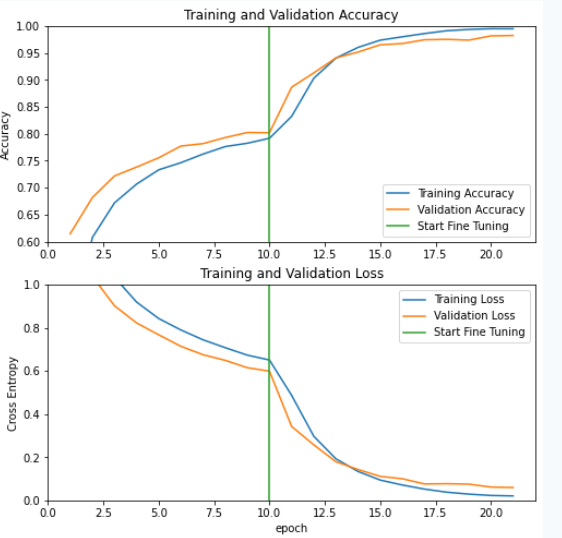
\includegraphics[width=8.5cm]{ModelCombineAccCEntropy.png}}
\caption{Model MobileNet v.2 with Adam Optimizer Combined dataset for Accuracy and Cross Entropy.}
\label{fig}
\end{figure}

%\begin{figure}[htbp]
%\centerline{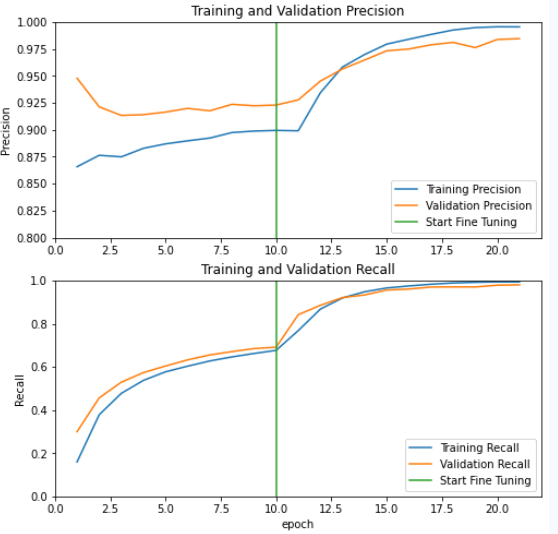
\includegraphics[width=8.5cm]{ModelCombinePrecisionRecall.png}}
%\caption{Model MobileNet v.2 with Adam Optimizer Indoor dataset for Precision and Recall.}
%\label{fig}
%\end{figure}

After the first training phase is over, some of the layers of the convolutional part are made trainable, in this case 100 of them are kept frozen and 56 are deemed trainable, bringing the number of trainable parameters up to 1,878,093. During the fine-tuning phase, a great improvement can be observed in all metrics analyzed, up to the 14 epochs when the results of the validation subset go under the training ones. 

\subsection{Indoor Segmented dataset}
The performance of models trained with segmented images and the original unsegmented version of the same images was compared. For the PlantVillage indoor laboratory dataset a model was trained on the original unsegmented version of the images using transfer learning with Inception-ResNet-v2. The model was trained for ten epochs before fine tuning. The test accuracy obtained was 94.38\%. The model was trained for another ten epochs with fine tuning. The test accuracy obtained was 98.37\%. Another model was trained on the segmented version of the same images using transfer learning with Inception-ResNet-v2. The model was trained for ten epochs before fine tuning. The test accuracy obtained was 92.50\%. The model was trained for another ten epochs with fine tuning. The test accuracy obtained was 96.88\%. The model trained on the original unsegmented data gave better test accuracy. In [4] for the PlantVillage dataset experiments are run on the segmented leaves. Segmentation removes any background information. The authors use AlexNet and GoogLeNet for transfer learning. In their experiments models trained with segmented images are found to give worse performance than those trained with the original unsegmented images. While we are using a pretrained model for transfer learning which is different from the pretrained models in their work our results are consistent with models trained on the original unsegmented images giving better performance. It is possible that some inherent bias is introduced into the dataset due to the background information.  \ 
\begin{figure}[htbp]
\centerline{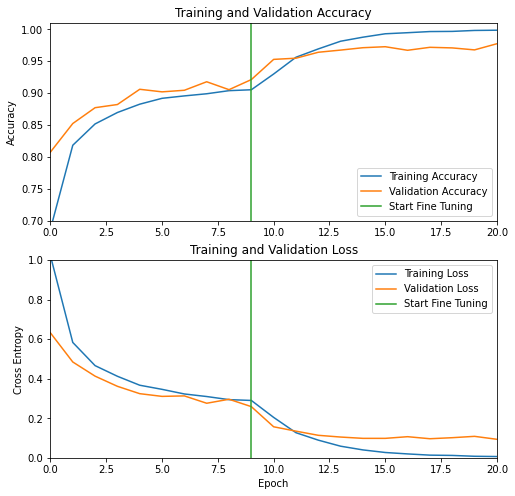
\includegraphics[width=8.5cm]{ModelIndoorsResNetEpochsSegmentedAccuracychart.png}}
\caption{Model InceptionResNet v.2 with Adam Optimizer Indoor Segmented dataset for Precision and Recall.}
\label{fig}
\end{figure}
 

\section{Results and Evaluation}
Here you should discuss how you used your methodology to answer the question.  How can you determine if your approach is good?  If you have to parameterise part of your approach, how have you done that, and why were these choices made?  What impacts can different parameterisations have  on  your  results?   You  should  also  discuss  the  results  in  detail  and discuss their impact and implications.  What do they show or not show? ”. \

How effective the models are in achieving the business objectives is assessed in the CRISP-DM evaluation phase. The models to evaluate should be Indoors images, Outdoor images with augmented train data and tested on the test data, Indoor and outdoor data combined, model to be tested on both random test subset and on the test outdoor data. Compared results will be then highlighted in the conclusion 
Also in this step a decision is made to either proceed to deployment or iterate further. 

The results shown in table III come from the model previously defined in methodology section Model Indoor dataset.  The model has been trained for 17 epochs in total, 10 where only the dense layer was trainable and 7 more epochs with 54 layers more trainable and a learning rate reduced by a factor of ten.  

\begin{table}[htbp]
\caption{Indoor Model}
\begin{center}
\begin{tabular}{|c|c|c|c|c|}
\hline
\textbf{Metrics}&\multicolumn{2}{|c|}{\textbf{Indoor Model}} \\
\cline{2-3} 
\textbf{Used} & \textbf{\textit{Indoor}}& \textbf{\textit{Outdoor}} \\
\hline
loss &0.058&9.788  \\
\hline
accuracy &0.981&0.075 \\
\hline
precision &0.982&0.083 \\
\hline
recall &0.978&0.075 \\
\hline
auc &0.999&0.537  \\
\hline
\multicolumn{3}{l}{$^{\mathrm{a}}$Over Indoor test and Outdoor test subsets.}
\end{tabular}
\label{tab1}
\end{center}
\end{table}

Included in Table III for the model trained on the augmented outdoor data with MobileNet and the Adam optimiser for 14 epochs are evaluation metrics obtained by applying the model to the outdoor test set and the indoor test set. The training accuracy and validation accuracy values for epoch 14 were 91.46\% and 91.28\% respectively. After epoch 14 the model starts to overfit the training data. From Table x it can be seen that the accuracy obtained on the indoor test set is 23.27\%, higher than the accuracy obtained on the outdoor test set 9.17\%. The precision, recall and AUC values for the indoor test set at 0.2779, 0.1945 and 0.6798 respectively are also higher than the precision, recall and AUC values for the outdoor test set at  0.1087, 0.0833 and 0.5952 respectively. 


\begin{table}[htbp]
\caption{Outdoor Model}
\begin{center}
\begin{tabular}{|c|c|c|c|c|}
\hline
\textbf{Metrics}&\multicolumn{2}{|c|}{\textbf{Outdoor Model}} \\
\cline{2-3} 
\textbf{Used} & \textbf{\textit{Indoor}}& \textbf{\textit{Outdoor}} \\
\hline
loss  &4.92 &3.70  \\
\hline
accuracy  &0.0917 &0.2327 \\
\hline
precision  &0.1087 &0.2779 \\
\hline
recall  &0.0833 &0.1945 \\
\hline
auc  &0.5952 &0.6798  \\
\hline
\multicolumn{3}{l}{$^{\mathrm{a}}$For the model trained on the augmented outdoor data.}
\end{tabular}
\label{tab1}
\end{center}
\end{table}

The model has been trained for 19 epochs, 10 with the training layer being only the dense layer and a learning rate of 0.001 and for 9 epochs on the fine-tuning phase, meaning that has 56 training layers, the ones in the dense layer plus 54 from the convolutional layers. The model produced is applied then to both testing subsets, one from the indoor model that contains 4026 samples and another from the outdoor subset  that contains 120 items. The results are shown in Table IV.
\begin{table}[htbp]
\caption{Combined Model}
\begin{center}
\begin{tabular}{|c|c|c|c|c|}
\hline
\textbf{Metrics}&\multicolumn{2}{|c|}{\textbf{Combined Model}} \\
\cline{2-3} 
\textbf{Used} & \textbf{\textit{Indoor}}& \textbf{\textit{Outdoor}} \\
\hline
loss  &9.024 &0.066   \\
\hline
accuracy  &0.092 &0.98  \\
\hline
precision  &0.098 &0.979  \\
\hline
recall  &0.092 &0.973  \\
\hline
auc  &0.542 &0.999   \\
\hline
\multicolumn{3}{l}{$^{\mathrm{a}}$Over Indoor test and Outdoor test subsets..}
\end{tabular}
\label{tab1}
\end{center}
\end{table}

There is a superior performance when the test in conducted over the indoor test subset, at 98\% virtually the same precision and a recall of 97.3\%. The area under the curve is almost total at 99.9\%. Comparing this outstanding performance with the performance achieved with the outdoor test subset, with accuracy and recall at 9.2\%, precision 9.8\%, the area under the curve at slightly over the half bring to two conclusions. First, that the performance in outdoor subset is basically what it can be achieved randomly, taking into consideration that there are 13 classes of. Second, that the performance is not improving by including more images in the training set. 

When the results of the 3 models are compared, 

\begin{figure}[htbp]
\centerline{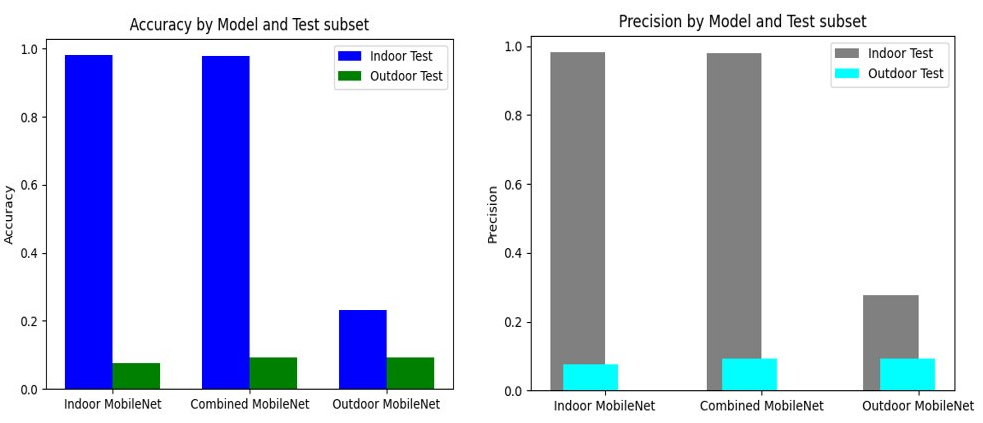
\includegraphics[width=8.5cm]{resultsPrecAccdifferentTests.png}}
\caption{Accuracy and Precision for the three models and tested on the indoors and outdoors test subsets.}
\label{fig}
\end{figure}

\section{Conclusion and Future Work}
The CRISP-DM final phase is deployment where the results of the data mining study are communicated to end users. This purpose is served by this report. The objectives of this study were met through the results. Knowledge discovery is the aim of CRISP-DM. This study accomplished this aim in a variety of ways. 

The lack of availability of images of leaves of diseased plants obtained outdoors in real world environments limited this study. Larger datasets of outdoor images would be of benefit for leaf disease classification. Also, in this study only three plant species were considered. In future work classification of plant disease from images could be extended to include additional plant species.

This study could be extended in a number of ways including through transfer learning using other pretrained CNN models to carry out image classification. In addition to the data augmentation techniques applied in this study other techniques could also be used including creating synthetic images of plant leaves using conditional generative adversarial networks. The Plant Doc outdoor images of leaves could be segmented and models, trained using these segmented images, compared against those trained using coloured versions of those images. We could extend this study from classifying the disease from the image of the leaf to grading how diseased the leaf is. In addition, we could compare the classification performance of the CNN models with that of other machine learning techniques. Our model could also be included as part of a pesticide prescription system for plant diseases. We could also compare the performance of a CNN model trained from scratch for classifying plant disease from leaf images against that of a CNN model trained by transfer learning. Our model could be used as part of a system to classify plant disease from images obtained using unmanned aerial vehicles. We could develop a lightweight model for devices with limited resources that still provides accurate performance in classifying plant disease from leaf images. The effect of varying the number of images used to train the models on the accuracy of classification could be investigated in future work.         


\bibliographystyle{IEEEtran}
\bibliography{references}

\end{document}
